\thispagestyle{doisongtoanhocnone}
\pagestyle{doisongtoanhoc}
\everymath{\color{doisongtoanhoc}}
\graphicspath{{../doisongtoanhoc/pic/}}
\blfootnote{$^1$\color{doisongtoanhoc}Theo thông báo Viện Hàn lâm Khoa học và Văn học Na Uy. https://abelprize.no/article/2023/luis-caffarelli-awarded-2023-abel-prize}
\begingroup
\AddToShipoutPicture*{\put(0,616){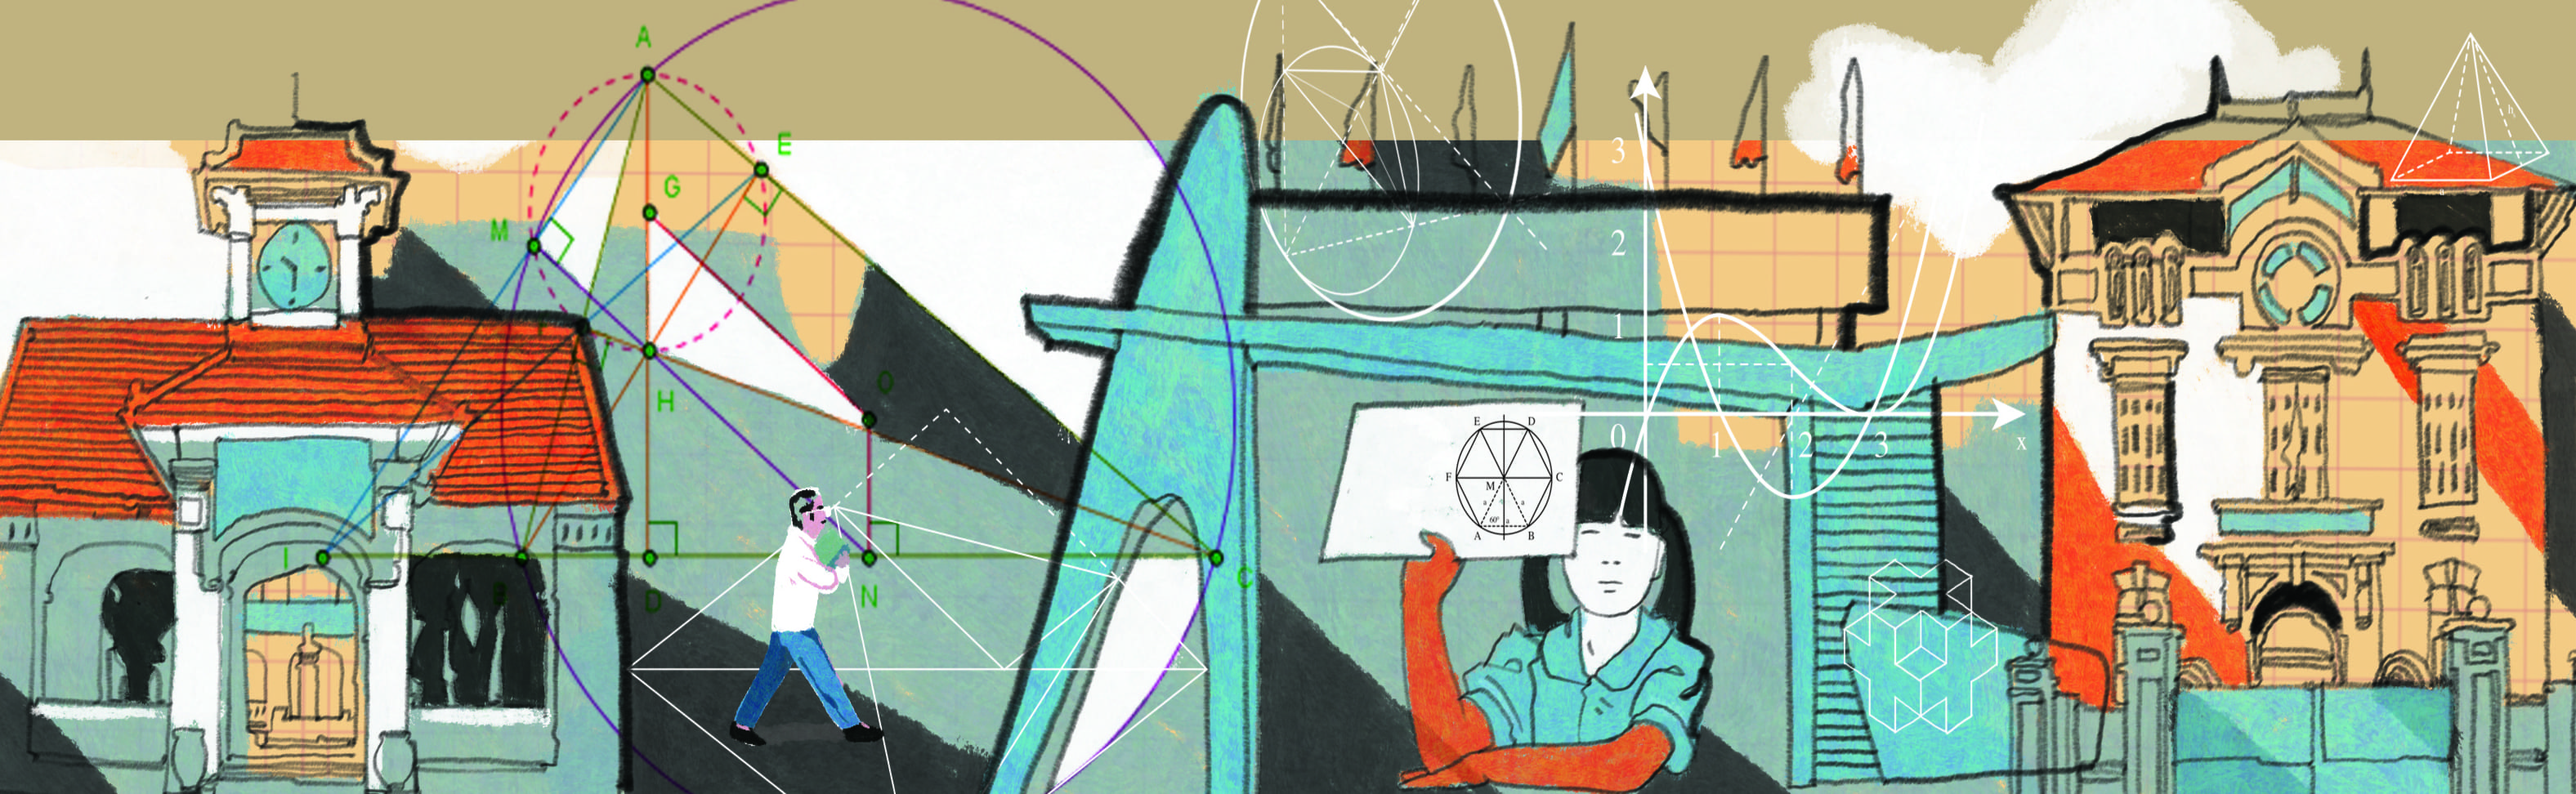
\includegraphics[width=19.3cm]{../bannerdoisong}}}
\AddToShipoutPicture*{\put(100,570){
\includegraphics[scale=0.95]{../tieude.pdf}}}\centering
\endgroup

\vspace*{140pt}


\begin{multicols}{2}	
	Luis A. Caffarelli được trao giải Abel $2023$ vì ``những đóng góp quan trọng cho lý thuyết chính quy của các phương trình đạo hàm riêng phi tuyến bao gồm các bài toán không có biên và phương trình Monge–Ampère.".
	\begin{figure}[H]
		\vspace*{-5pt}
		\centering
		\captionsetup{labelformat= empty, justification=centering}
		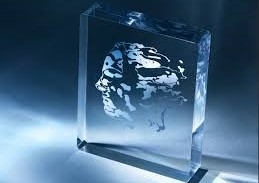
\includegraphics[width= 1\linewidth]{1}
		\vspace*{-15pt}
	\end{figure}
	Phương trình vi phân là công cụ mà các nhà khoa học sử dụng để dự đoán hành vi của thế giới vật chất. Các phương trình này liên quan đến một hoặc nhiều hàm chưa biết và đạo hàm của chúng. Các hàm thường đại diện cho các đại lượng vật lý, các đạo hàm đại diện cho tốc độ thay đổi của chúng và phương trình vi phân xác định mối quan hệ giữa hai đại lượng này. Những mối quan hệ như vậy là phổ biến; do đó, các phương trình vi phân đóng một vai trò nổi bật trong nhiều ngành bao gồm kỹ thuật, vật lý, kinh tế và sinh học.
	\vskip 0.1cm
	Các phương trình đạo hàm riêng phát sinh một cách tự nhiên như các quy luật của Tự nhiên, để mô tả các hiện tượng khác nhau như dòng chảy của nước hoặc sự phát triển của dân số. Những phương trình này luôn là nguồn nghiên cứu mãnh liệt kể từ thời của Isaac Newton và Gottfried Leibniz. Tuy nhiên, bất chấp những nỗ lực đáng kể của nhiều nhà toán học trong nhiều thế kỷ, các câu hỏi cơ bản liên quan đến sự tồn tại, tính duy nhất, tính chính quy và tính ổn định của các nghiệm của một số phương trình quan trọng vẫn chưa được giải quyết.
	\begin{figure}[H]
		\vspace*{-5pt}
		\centering
		\captionsetup{labelformat= empty, justification=centering}
		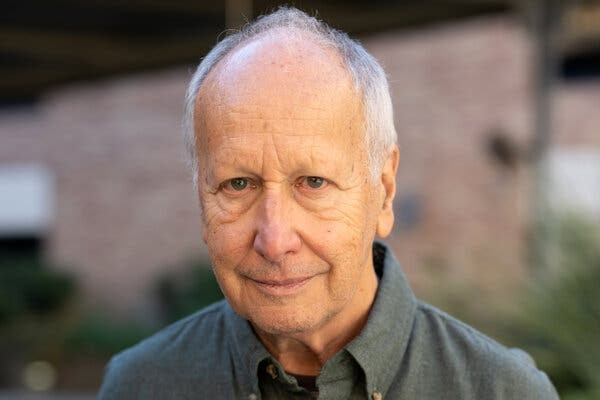
\includegraphics[width= 1\linewidth]{2}
		\caption{\small\textit{\color{doisongtoanhoc}Ảnh: Nolan Zunk, Đại học Texas ở Austin.}}
		\vspace*{-10pt}
	\end{figure}
	\textbf{\color{doisongtoanhoc}Kết quả chuẩn mực về kỹ thuật}
	\vskip 0.1cm
	Rất ít nhà toán học đương đại khác có đóng góp nhiều hơn cho sự hiểu biết của chúng ta về phương trình đạo hàm riêng so với Luis Caffarelli, một người Mỹ gốc Argentina. Ông đã đưa ra những kỹ thuật mới tài tình, thể hiện cái nhìn sâu sắc về hình học và tạo ra nhiều kết quả có ảnh hưởng. Trong khoảng thời gian hơn $40$ năm, ông đã có những đóng góp đột phá cho lý thuyết về tính chính quy. Tính chính quy -- hay độ trơn -- của các nghiệm là điều cần thiết trong tính toán số, và sự vắng mặt của tính đều đặn là thước đo mức độ Tự nhiên có thể hành xử dữ dội như thế nào.
	\vskip 0.1cm
	Helge Holden, chủ tịch Ủy ban Abel, cho biết: ``Các định lý của Caffarelli đã thay đổi hoàn toàn hiểu biết của chúng ta về các lớp phương trình đạo hàm riêng phi tuyến với nhiều ứng dụng. Các kết quả là chuẩn mực về mặt kỹ thuật, ảnh hưởng tới nhiều lĩnh vực khác nhau của toán học và các ứng dụng của nó." 
	\vskip 0.1cm
	Phần lớn công việc của Luis A. Caffarelli liên quan đến các bài toán không có biên.  Ví dụ, hãy xem xét vấn đề băng tan thành nước. Ở đây biên là giao diện giữa nước và băng; nó là một phần của ấn số cần được xác định. Một ví dụ khác là nước thấm qua một môi trường xốp -- một lần nữa, giao diện của nước và môi trường cần được hiểu rõ. Caffarelli đã đưa ra các giải pháp thâm nhập cho những vấn đề này với các ứng dụng cho các giao diện rắn--lỏng, dòng phun và tạo bọt, dòng khí và chất lỏng trong môi trường xốp, cũng như toán tài chính.
	\vskip 0.1cm
	\textbf{\color{doisongtoanhoc}Ảnh hưởng to lớn đến lĩnh vực}
	\vskip 0.1cm
	Caffarelli là một nhà toán học có hiệu suất đặc biệt, với hơn $130$ cộng sự và hơn $30$ nghiên cứu sinh trong khoảng thời gian $50$ năm.
	\vskip 0.1cm
	Helge Holden nói: ``Kết hợp sự hiểu biết sâu sắc về hình học với các công cụ và phương pháp phân tích khéo léo mà ông ấy đã và tiếp tục có ảnh hưởng to lớn đến lĩnh vực này.
	\vskip 0.1cm
	Luis A. Caffarelli đã giành được nhiều giải thưởng, trong đó có Giải thưởng Leroy P. Steele cho Thành tựu Trọn đời về Toán học, Giải thưởng Wolf và Giải thưởng Shaw.
\end{multicols}
